\section{Workload Analysis}

In this section, we analyze traces from a variety of production
file systems which includes storage systems for enterprise,
high performance computing (HPC), and
data-intensive computing (DISC).
The traces we analyzed are either reproduced from previous works
\cite{brent13, Bill11, Fan11} or collected by ourselves.
These storage systems include engineering desktops from Microsoft
\cite{Bill11}, 65 customer installations from Panasas \cite{brent13},
Hadoop clusters from Yahoo!, Facebook, LinkedIn and CMU OpenCloud.
The size of storage systems in the traces
range from one single machine to thousands of machines.

We collected both static and dynamic metadata samples.
Static metadata includes file size distribution,
file counts in directories, and path depth which shows
the statistics of the file system at rest.
Dynamic metadata is about the workloads applied to the system,
for example, percentage of different operations,
locality in the pathnames and so on.

Our objective behind analyzing these traces is to
high-light characteristics –
heavy tail distribution of directory size and file size,
and logarithmic growth of directory depth -
that motivates our design choices of scalable metadata service.

\subsection{Heavy-Tailed Directory Sizes}
File system namespace exhibits a heavy-tailed distribution
of directory size. Typically, a file system consists of
many small directories and relatively few large directories.
Figure \ref{fig:directory_size} shows the median, 90-percentile,
and maximum directory size of all collected storage system samples.
About 60 out of 70 file systems that are collected in our traces
have nearly $90\%$ directories with size fewer than 128.
On the other hand, large directories continue to grow with
the increasing size of the storage system. Figure \ref{fig:large_directory}
shows such growing trend. Many parallel computing applications
are reported to require concurrent access to these large directories
such as check pointing, and map-reduce jobs \cite{PLFS, MapReduce}.
Therefore, a scalable metadata service
should support a large amount of small objects, as well as
efficient distribution of large directory for concurrent access.


\begin{figure}[!ht]
\center
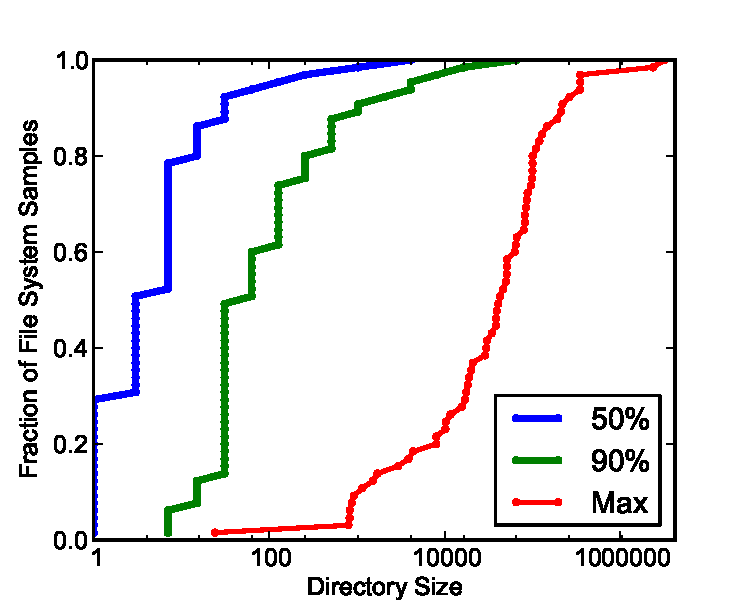
\includegraphics[scale=0.5]{figs/directory_size}
\caption{\textit{The median, 90-percentile,
and maximum directory sizes of collected file system samples.
}}
\label{fig:directory_size}
\end{figure}

\begin{figure}[!ht]
\center
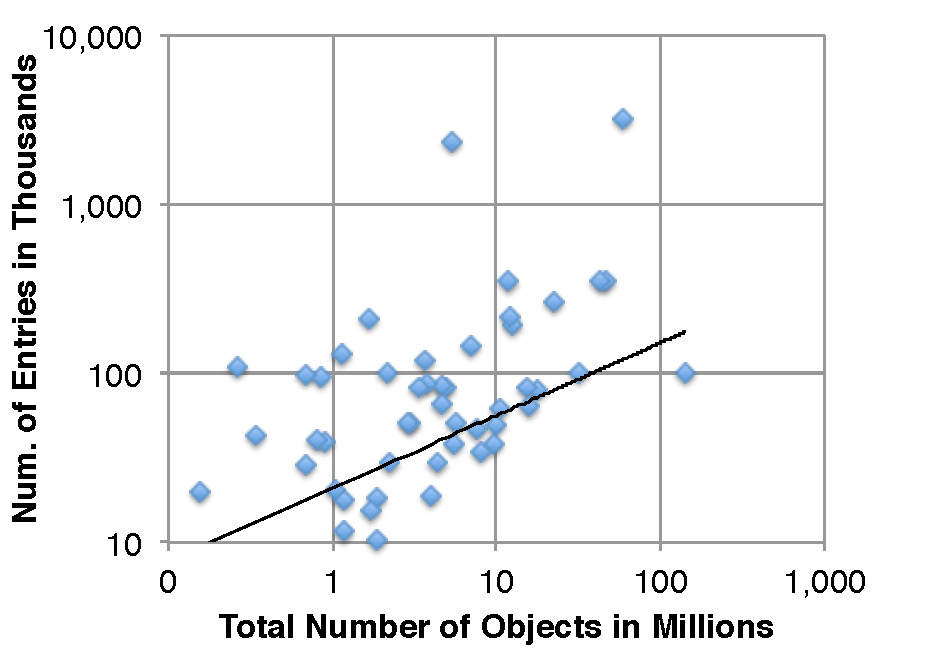
\includegraphics[scale=0.4]{figs/large_dir}
\caption{\textit{The relation between the size of the largest file system
and the size of the file system (measured in total number of objects).}}
\label{fig:large_directory}
\end{figure}

Regarding to the tree structure, we also found that the average depth
of the tree does not increase too much as the system grows.
Figure \ref{fig:directory_depth} shows directory tree
depth statistics of some file systems in our traces
(this information is not available for Panasas customer installations).
Most file systems have 90\% directories with depth lower than 16.
We conjecture that

\begin{figure}[!ht]
\center
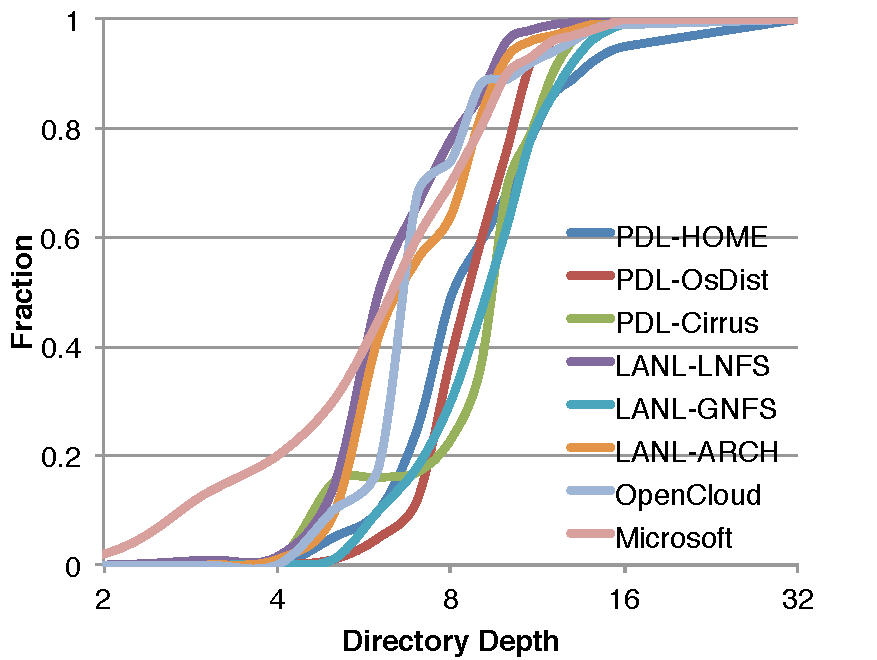
\includegraphics[scale=0.4]{figs/directory_depth}
\caption{}
\label{fig:directory_depth}
\end{figure}

\subsection{Highly-Skewed File System Operations}

%\subsection{Small Files are Popular}
\begin{figure}[!ht]
\center
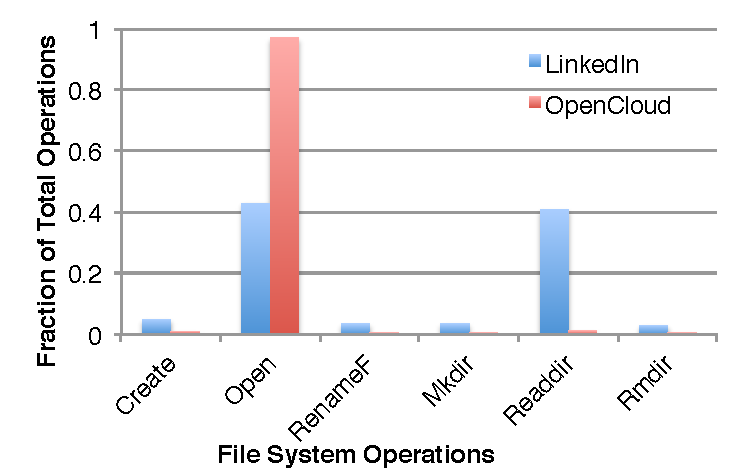
\includegraphics[scale=0.5]{figs/operation_distribution}
\caption{}
\label{fig:operation}
\end{figure}


